\documentclass[a4paper,12pt]{article}
\usepackage[utf8]{inputenc}
\usepackage[english]{babel}
\usepackage{graphicx}
\usepackage{amsmath}
\usepackage{amssymb}
\usepackage{hyperref}
\usepackage{geometry}
\usepackage{tabularx}
\usepackage{float}
\usepackage[backend=biber, style=numeric, sorting=none]{biblatex}
\usepackage{booktabs}
\usepackage{colortbl}
\usepackage{xcolor}
\usepackage{caption} % For customizing captions


% Set the caption font size
\captionsetup{font=small}


\addbibresource{references.bib}

\geometry{a4paper, left=25mm, right=25mm, top=25mm, bottom=25mm}
\title{Project 1: Supervised Learning - Classification}
\author{Alexander Svarfdal Gudmundsson \and Jan Babin}
\date{\today}

\begin{document}

\maketitle

\section{Introduction}
\subsection{Background}
Diabetes is a chronic condition characterised by elevated blood sugar levels. While genetic factors 
can play a role, a significant amount of diabetes Type 2 cases is associated with lifestyle choices. 
According to the World Health Organization \cite{WHO2016}, 422 million people worldwide 
are living with diabetes, with numbers continuing to rise. The societal impact of diabetes is 
significant: a diminished quality of life and a higher risk of serious health complications which in 
turn may lead to increased healthcare costs. Therefore, there is medical merit in
early predictions of diabetes to refine treatment and management strategies.

\subsection{Objective}
The goal of this project is to build a machine learning model that can identify 
patterns in lifestyle and demographic data associated with diabetes and thereby predict whether
a given person has diabetes / is very likely do develop it. While the 
model is purely intended for academic purpose, the project allows us to 
explore how machine learning can be used to analyse health-related data and 
provide insights into potential risk factors.

\subsection{Dataset}
The dataset at hand, "Diabetes, Hypertension and Stroke Prediction," is from Kaggle and contains 
health-related data in CSV format intended for predicting diabetes, hypertension and stroke. 
For this project, we are solely focussing on diabetes. The dataset consists of 70,692 observations 
and 18 features, some of which are outlined as follows (for a full overview, see Table \ref{tab:feature_list} in the Appendix):
\begin{itemize}
    \item \textbf{Age}: Coded in 13 age groups (see Figure \ref{fig:age_groups}).
    \item \textbf{Sex}: Binary variable representing male (0.0) and female (1.0).
    \item \textbf{BMI}: Body Mass Index, a continuous variable.
    \item \textbf{Lifestyle indicators}: Such as smoking status (whether the individual has smoked 
    at least 100 cigarettes in their lifetime), physical activity in the past 30 days 
    (excluding job-related activity), daily fruit and vegetable consumption, and heavy alcohol 
    consumption (based on defined weekly limits for men and women).
    \item \textbf{General health and mental/physical health}: Self-reported general health on a 
    scale from 1 (excellent) to 5 (poor), along with the number of days with poor mental and 
    physical health over the past 30 days.
    \item \textbf{Pre-existing conditions}: Information on high cholesterol, coronary heart 
    disease or myocardial infarction, and difficulty walking.
\end{itemize}

\begin{figure}[h!]
    \centering
    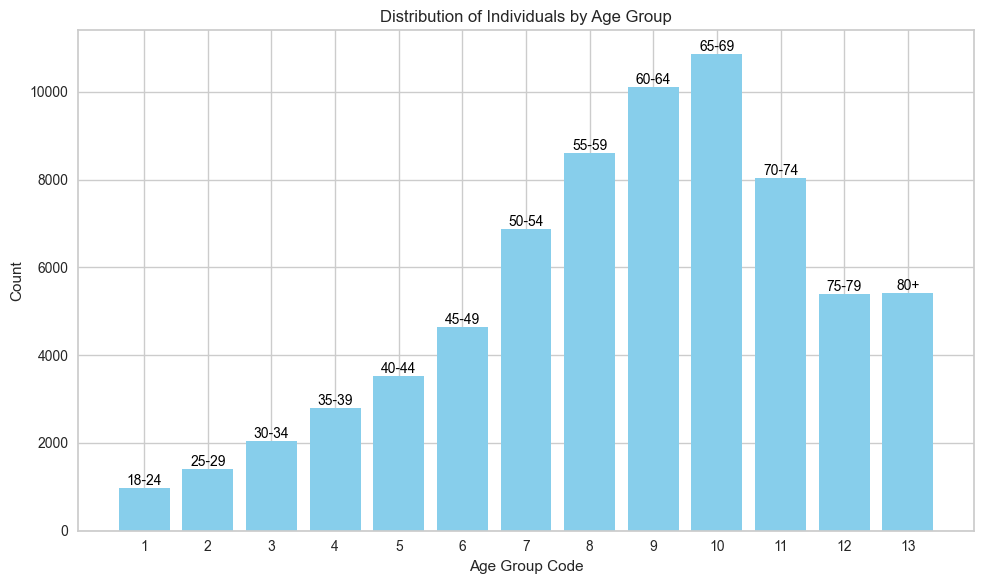
\includegraphics[width=0.7\textwidth]{plot_age_groups.png}
    \caption{Distribution of Age Groups in the Dataset: Counts of individuals across thirteen defined age groups, 
    ranging from 18 to 24 years to 80 years and older, according to the AGEG5YR scheme.}
    \label{fig:age_groups}
\end{figure}

The target variable is \textbf{Diabetes}, which is represented as a binary category 
(0.0 for no diabetes, 1.0 for diabetes). No missing or null values were identified in the dataset, 
ensuring that data cleaning was minimal and straightforward. Furthermore, the dataset is perfectly 
balanced, in that, 50\% of observations correspond to diabetes, the other 50\% do not.


\section{Process}
The steps involved in the analysis follow a standard supervised machine learning pipeline, 
from data preparation to model selection and evaluation.

\section{CHECK FOR HIGH COLESTEROL AND DIABETES, part of EDA.}

\subsection{Data Loading and Exploration}
The dataset was loaded into a pandas DataFrame. Initial exploration was conducted to understand 
the structure of the data:
\begin{itemize}
    \item Data Integrity: We confirmed that the dataset contained no missing or null values.
    \item Feature Exploration: The features were analysed for their unique values and data 
    types, revealing that many variables were binary, and the rest were either categorical or 
    continuous. Continuous variables included features like BMI, Age, MentHlth, and PhysHlth, 
    while categorical variables included GenHlth (self-reported health scale from 1 to 5) 
    and binary indicators for lifestyle factors like Smoking, Physical Activity, and Alcohol 
    Consumption.
\end{itemize}

\subsection{Preprocessing}
\subsubsection{One-Hot Encoding}
Since the data set's features were numeric, we tried one-hot encoding features that seemed categorical
into binary columns to prevent the model from interpreting these as continuous data, where actually
the difference between values might not bear any meaning. 


\subsubsection{Scaling}
Certain features with a wide range of values were standardized using StandardScaler. These included:
BMI, MentHlth, PhysHlth, and Age: Standardization ensures that the models 
(e.g., logistic regression, support vector machines) are not biased towards features with larger 
numeric ranges. This is important for algorithms that rely on the magnitude of features during 
decision-making.

\subsubsection{Train-Test Split}
The dataset was split into a training set (80\%) and a test set (20\%) using train\_test\_split from 
sklearn. We decided on this split for our relatively large data set in order to retrieve both substantial 
training and test set sizes. This reduces overfitting (model has enough training to learn nuances without 
memorising specific instances) as well as yielding a robust set of unseen data for unseen data and is a common industry practice. 
Stratification was applied to ensure that the class distribution of the target variable 
(Diabetes) remained balanced across the training and test sets.

\subsection{Feature Correlation Analysis}
To explore potential multicollinearity among features, a correlation matrix was generated using 
Seaborn's heatmap function. The goal was to identify highly correlated features that could negatively 
impact model performance by redundancy. [ADD SOME INFO ABOUT PEARSON CORRELATION]

\subsection{Model Selection and Evaluation}
\subsubsection{PyCaret Experiment Setup}
For model selection, we utilised PyCaret's \texttt{ClassificationExperiment} to quickly get a 
comparison between multiple classification models. The \texttt{ClassificationExperiment} tries 
different models to rank the models based on accuracy, using default hyperparameters based on common practice. 
We then selected the 5 best performing models to fine-tune further via hyperparameter optimisation. 
\\
PyCaret’s built-in random grid-search was used to tune the hyperparameters of the selected models, 
optimising for accuracy. The random grid search works by 
randomly choosing a parameter value from a given (or a default) range. It then tries out different random combinations
of hyperparameters and chooses the best one based on accuracy.

\subsubsection{Model Stacking and Ensembling}
In an effort to improve prediction accuracy, ensemble learning methods were applied:
\begin{itemize}
    \item A hard voting ensemble (that is, majority vote) \texttt{(blend\_models)} was created using the 
    5 top-performing models chosen previously. The resulting blended model runs the base models on an input
    and will output whatever was predicted most often among these.
    \item Furthermore, a combined model using stacking was also built. 
    Stacking works by training a model to aggreagate the predictions of all of the predictors. 
    
\end{itemize} 

\subsubsection{Feature Selection}
Some rudimentary feature selection was employed, using PyCaret's \texttt{ClassificationExperiment}'s inbuilt
feature selection method. This reduces the set of features to only those deemed important based on
statistical tests and feature importance techniques, which may help improve model performance.

\section{Results}
By using PyCaret's built-in \texttt{ClassificationExperiment}, we can quickly evaluate which classifiers perform best on our training dataset.


However, the stacking model did not outperform the ensemble.
After experimenting with feature selection (also implemented via PyCaret), we found that applying 
feature selection resulted in slightly lower model performance. Therefore, the final models were 
built without this step.

\subsection{TBD}
Findings: The GenHlth and PhysHlth features exhibited some degree of linear correlation but it was
not high enough to justify omitting one of two would outweigh having more features / data to train 
on.
WE MIGHT WANNA REFERENC SOMETHING REGARDING CORRELATION VALUES HERE 
(when to throw away a feature / when not)

\begin{figure}[H]
    \centering
    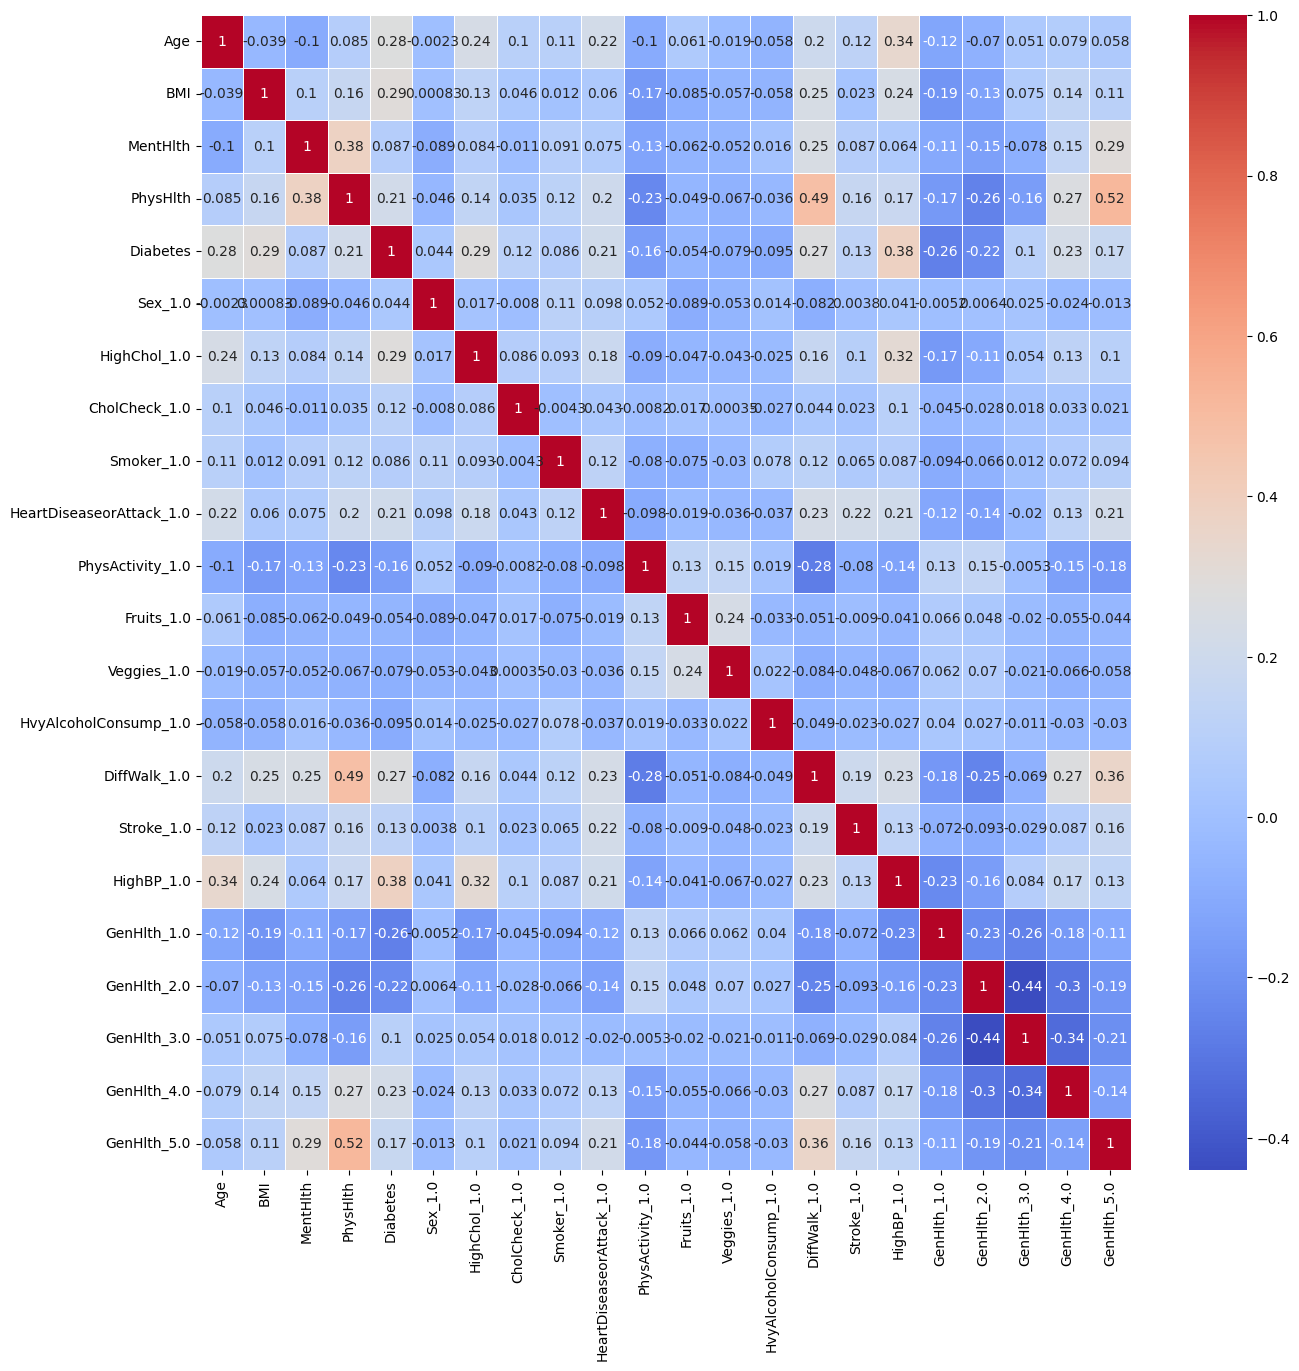
\includegraphics[width=0.7\textwidth]{correlation_matrix.png}
    \caption{Correlation matrix showing relationships between features in the dataset (Pearson correlation). 
    Higher values indicate stronger correlations.}
    \label{fig:correlation_matrix}
\end{figure}

\begin{itemize}
    \item Sex: Encoded as a binary variable with one-hot encoding and drop\_first=True to prevent
    perfect multicollinearity (i.e., avoiding redundancy with one binary variable sufficing to 
    represent gender).
    \item GenHlth: This feature, originally a categorical variable on a scale from 1 to 5, 
    was one-hot encoded to allow for better model interpretation and training.
\end{itemize}

\begin{table}[h!]
\centering
\begin{tabular}{l l c c c c}
\toprule
\textbf{Model} & \textbf{Classifier} & \textbf{Accuracy} & \textbf{Recall} & \textbf{Precision} & \textbf{F1} \\
\midrule
\texttt{gbc} & Gradient Boosting Classifier & \cellcolor{yellow}0.7508 & 0.7897 & 0.7329 & \cellcolor{yellow}0.7601 \\
\texttt{lightgbm} & Light Gradient Boosting Machine & 0.7495 & \cellcolor{yellow}0.7926 & 0.7298 & 0.7598 \\
\texttt{ada} & Ada Boost Classifier & 0.7482 & 0.7731 & \cellcolor{yellow}0.7366 & 0.7543 \\
\texttt{lr} & Logistic Regression & 0.7467 & 0.7737 & 0.7342 & 0.7534 \\
\texttt{ridge} & Ridge Classifier & 0.7467 & 0.7799 & 0.7314 & 0.7549 \\
\texttt{lda} & Linear Discriminant Analysis & 0.7467 & 0.7798 & 0.7314 & 0.7548 \\
\texttt{rf} & Random Forest Classifier & 0.7273 & 0.7627 & 0.7124 & 0.7366 \\
\texttt{nb} & Naive Bayes & 0.7246 & 0.7251 & 0.7244 & 0.7247 \\
\texttt{et} & Extra Trees Classifier & 0.7108 & 0.7330 & 0.7019 & 0.7171 \\
\texttt{knn} & K Neighbors Classifier & 0.7019 & 0.7196 & 0.6951 & 0.7071 \\
\bottomrule
\end{tabular}
\caption{Performance of Top 10 Models (Accuracy, Recall, Precision, F1) with Highlighted Values}
\label{tab:model_performance}
\end{table}
\subsection{Summary of Best Model Performance}



The table below shows the best results for the top 5 models (sorted by accuracy) for the key metrics: Accuracy, Recall, Precision, and F1. The best value for each metric is highlighted in yellow.
WE NEED TO CHECK IF THIS IS RIGHT
\begin{table}[h!]
\centering
\begin{tabular}{l l c c c c}
\toprule
\textbf{Model} & \textbf{Classifier} & \textbf{Accuracy} & \textbf{Recall} & \textbf{Precision} & \textbf{F1} \\
\midrule
\texttt{lightgbm} & Light Gradient Boosting Machine & \cellcolor{yellow}0.7515 & \cellcolor{yellow}0.7930 & 0.7336 & \cellcolor{yellow}0.7603 \\  % Tuned selected based on accuracy
\texttt{gbc}    & Gradient Boosting Classifier & 0.7508 & 0.7897 & 0.7329 & 0.7601 \\  % Original selected based on accuracy
\texttt{lr}     & Logistic Regression & 0.7499 & 0.7737 & 0.7342 & 0.7534 \\  % Tuned selected based on accuracy
\texttt{ada}    & Ada Boost Classifier & 0.7482 & 0.7731 & \cellcolor{yellow}0.7366 & 0.7543 \\  % Original selected based on accuracy
\texttt{ridge}  & Ridge Classifier & 0.7467 & 0.7799 & 0.7314 & 0.7549 \\  % Original selected based on accuracy
\bottomrule
\end{tabular}
\caption{Best Results of Top 5 Models (Sorted by Accuracy, with highlights for best metrics)}
\label{tab:best_model_performance}
\end{table}
\subsection{Ensamble (stacking and blending)}
\subsection{Testing the models with the test data}
\subsection{Overfitting/Underfitting}
\subsection{Addressing over and underfitting?}

\section{Future Work}
% https://www.kaggle.com/code/solafajobi/diabetes-perfect-prediction#Feature-Selection

seems to get better results, check stuff he did

\clearpage

\appendix
\section*{Appendix}

\begin{table}[h!]
    \centering
    \begin{tabularx}{\textwidth}{|l|X|}
    \hline
    \textbf{Feature} & \textbf{Description} \\ \hline
    Age & Coded in 13 age groups (e.g., 1: 18-24, 2: 25-29, etc.) \\ \hline
    Sex & Sex of the individual (0: Male, 1: Female) \\ \hline
    HighChol & High cholesterol (0: No, 1: Yes) \\ \hline
    CholCheck & Checked cholesterol in the last 5 years (0: No, 1: Yes) \\ \hline
    BMI & Body Mass Index (continuous variable) \\ \hline
    Smoker & Smoked at least 100 cigarettes in their lifetime (0: No, 1: Yes) \\ \hline
    HeartDiseaseorAttack & History of coronary heart disease or myocardial infarction (0: No, 1: Yes) \\ \hline
    PhysActivity & Engaged in physical activity in the past 30 days, excluding work (0: No, 1: Yes) \\ \hline
    Fruits & Consumes fruit 1 or more times per day (0: No, 1: Yes) \\ \hline
    Veggies & Consumes vegetables 1 or more times per day (0: No, 1: Yes) \\ \hline
    HvyAlcoholConsump & Heavy alcohol consumption (men: 14+ drinks/week, women: 7+ drinks/week) (0: No, 1: Yes) \\ \hline
    GenHlth & Self-reported general health (1: Excellent, 2: Very good, 3: Good, 4: Fair, 5: Poor) \\ \hline
    MentHlth & Days of poor mental health in the past 30 days (0 to 30) \\ \hline
    PhysHlth & Days of poor physical health in the past 30 days (0 to 30) \\ \hline
    DiffWalk & Difficulty walking or climbing stairs (0: No, 1: Yes) \\ \hline
    Stroke & History of stroke (0: No, 1: Yes) \\ \hline
    HighBP & High blood pressure (0: No, 1: Yes) \\ \hline
    Diabetes & Presence of diabetes (0: No, 1: Yes) \\ \hline
    \end{tabularx}
    \caption{Full list of dataset features used in the analysis.}
    \label{tab:feature_list}
\end{table}

\printbibliography

\end{document}